\documentclass[10pt,usenames,dvipsnames]{beamer}

\newcommand{\lectnum}{L15}
\newcommand{\lecttitle}{Ensemble methods}

\usepackage{amsmath, amssymb, graphicx}
\usepackage[]{algorithm2e}
\usepackage{pdfpages}
\usepackage[british]{babel}

\hypersetup{colorlinks,linkcolor=,urlcolor=blue}
\newenvironment{titledslide}[1]{\begin{frame}\frametitle{#1}}{\end{frame}}

\mode<presentation>{\setbeamercovered{transparent}}

\setbeamertemplate{sidebar right}{}
\setbeamertemplate{footline}{%
\hfill\usebeamertemplate***{navigation symbols}
\hspace{0.4cm}\lectnum: \insertframenumber{}/\inserttotalframenumber \hspace*{0.4cm}}

\author{James Cussens}

\title{COMS30035, Machine learning:\\ \vspace{5pt} \lecttitle}

\institute{School of Computer Science\\University of Bristol}

\begin{document}
%%%%%%%%%%%%%%%%%%%%%%%%%%%%%%%%%%%%%%%%%%%%%%%%%%%%%%%%%%%%%%%%%%%%%%

\begin{frame}
  \titlepage
\end{frame}

%%%%%%%%%%%%%%%%%%%%%%%%%%%%%%%%%%%%%%%%%%%%%%%%%%%%%%%%%%%%%%%%%%%%%%



%%%%%%%%%%%%%%%%%%%%%%%%%%%%%%%%%%%%%%%%%%%%%%%%%%%%%%%%%%%%%%%%%%%%%%
\begin{titledslide}{Acknowledgement}

  \begin{itemize}
  \item These slides are adapted from ones originally created by Edwin Simpson. 
  \end{itemize}
  
\end{titledslide}


\begin{frame}[fragile]
\frametitle{Agenda}   % expectation: 33 slides + title and agenda, 11 slides per chunk
\begin{itemize}
\item Model Selection
\textcolor{gray}{\item Model Averaging
\item Ensembles: Bagging
\item Ensembles: Boosting and Stacking}
\item \textcolor{gray}{Tree-based Models} 
\item \textcolor{gray}{Conditional Mixture Models  
\item Ensembles of Humans}  
\end{itemize}
\end{frame}

\begin{frame}[fragile]
\frametitle{The Model Selection Problem}
% img: a whole bunch of different models?
\begin{itemize}
% There are multiple different models that we could train and apply to any given task, so how do we decide which to use?
\item Select a model $h$ from a set of possible models in a set $H$, 
\uncover<2->{\item The models in $H$ can differ in various ways, such as:}
	\begin{itemize}
	\uncover<3->{\item The structure of the model, e.g., differences in graphical models;}
	\uncover<4->{\item The choice of prior distribution $p(\theta)$ over model parameters;}
	\uncover<5->{\item The learning algorithm used, e.g., EM, MCMC, backpropagation,;}
	\uncover<5->{\item Parameters of the learning algorithm, like learning rate for stochastic gradient descent (SGD);}
	\uncover<6->{\item The features of the data used as inputs to the model;}
	\uncover<7->{\item The examples in the dataset the model is trained on;}
	\uncover<8->{\item Random initialisation of parameters for EM or SGD}
	\end{itemize}
%\item For any characteristic that we cannot learn through training or inference is part of the model selection problem.
%\item Several different data-driven techniques can help us to \emph{select} a model...
%\item Or we can \emph{combine} models, which often leads to better performance (more on this later!)!  % more on why this works later
\end{itemize}
\end{frame}



\begin{frame}
\frametitle{Hyperparameters}
%include a plot here?
\begin{tikzpicture}[classical/.style={thick,double,<->,shorten >=0pt,shorten <=0pt,>=stealth},
flow/.style={thick, gray, decoration={markings,mark=at position
   1 with {\arrow[thick,gray]{ triangle 60}}},
   double distance=6.5pt, shorten >= 6.5pt,
   preaction = {decorate, gray},
   postaction = {draw,line width=7pt, gray,shorten >= 6.3pt}},
    mynode/.style={rectangle,rounded corners,draw=black, top color=white, bottom color=blue!50, thin, inner sep=0.25em, minimum size=0.1em, text centered},
    dep/.style={, ->, >=stealth'}]

\node[draw=none] (2) at (1,1.2) {}; % model selection
\node[draw=none] (4) at (4,1.2) {}; % inference/training 
\node[draw=none] (6) at (7,1.2) {}; % inference/prediction
\node[draw=none] (8) at (10,1.2) {}; % evaluation 
    
\node[draw=none]  at (1,0) {hyperparameters}; % model selection
\node[draw=none]  at (4,0) {parameters}; % inference/training 
\node[draw=none]  at (7,0) {predictions}; % inference/prediction
\node[draw=none]  at (10,0) {score}; % evaluation 

\node[draw,mynode] (1) at (1,2.2) {model selection}; % model selection
\node[draw,mynode] (3) at (4,2.2) {training}; % inference/training 
\node[draw,mynode] (5) at (7,2.2) {prediction}; % inference/prediction
\node[draw,mynode] (7) at (10,2.2) {evaluation}; % evaluation 

\draw[classical] (1) to (2);
\draw[classical] (3) to (4);
\draw[classical] (5) to (6);
\draw[classical] (7) to (8);

\draw[flow] (2) to (3);
\draw[flow] (4) to (5);
\draw[flow] (6) to (7);

% hyperparameters
\node[inner sep=0pt] at (0.5, 0.75) {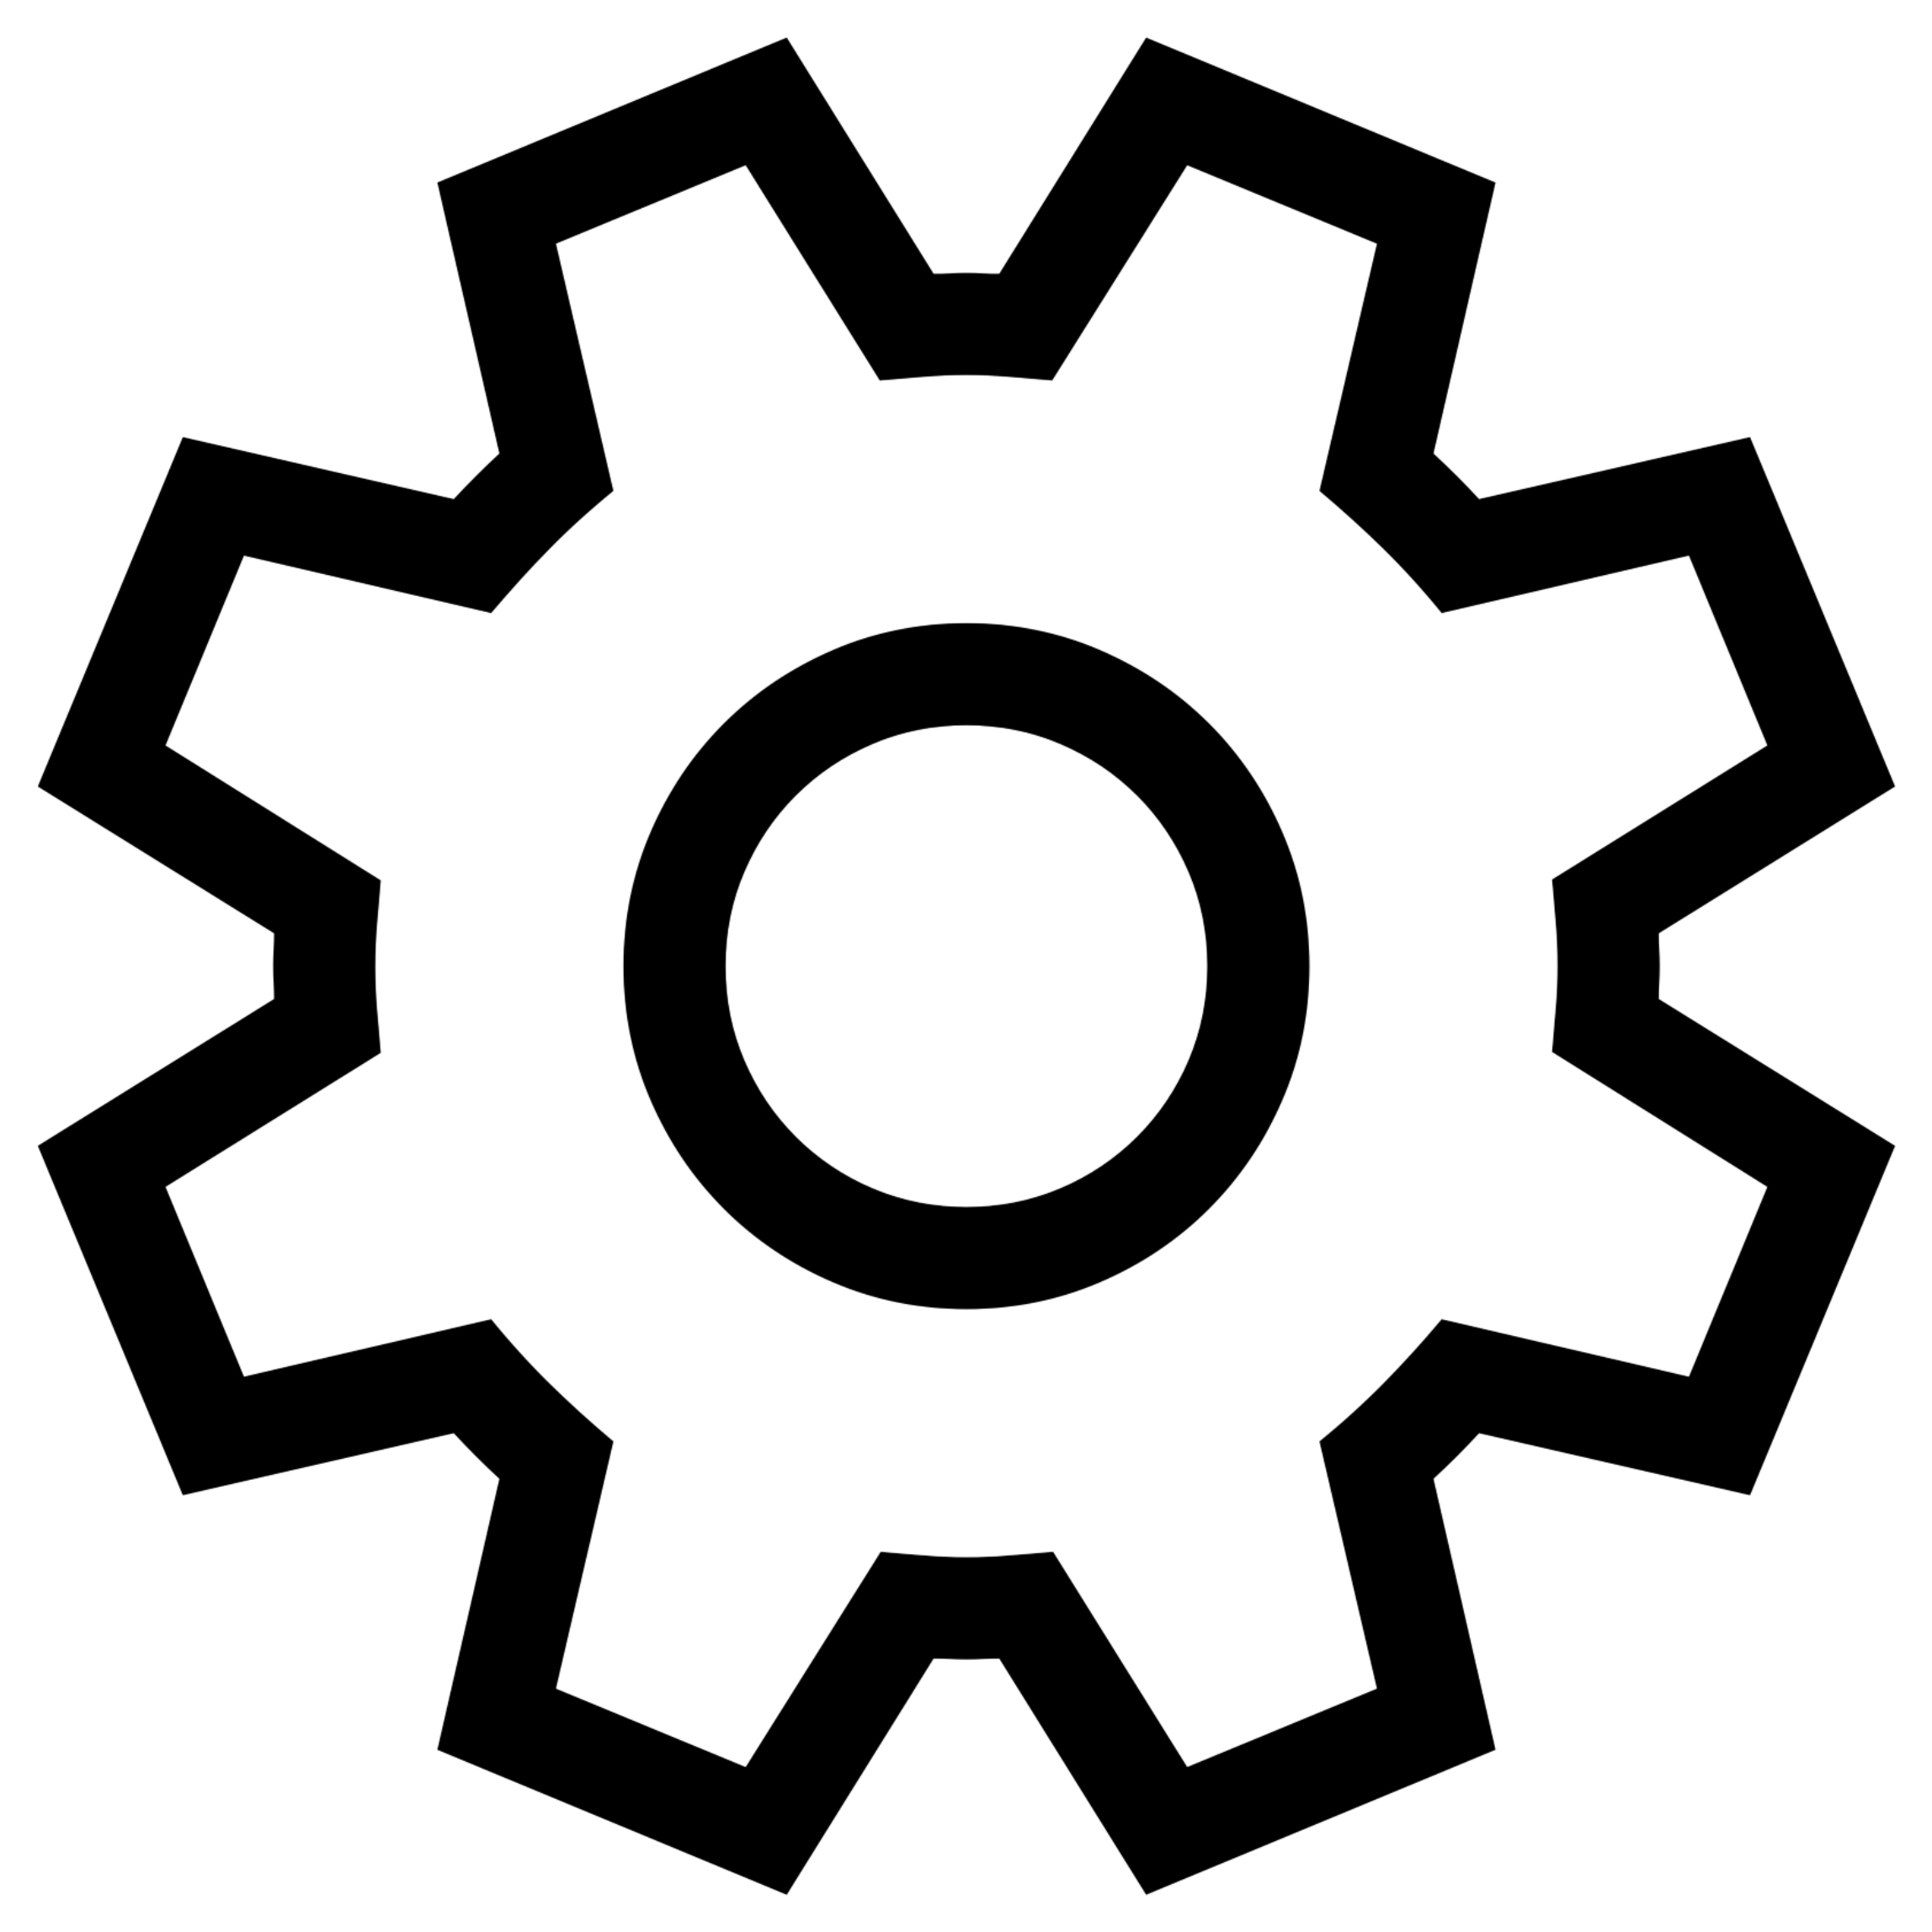
\includegraphics[scale=0.04]{../figures/Windows_Settings_app_icon.png} };
\node[draw=none,inner sep=1pt,anchor=west]  at (1,1) {\scriptsize $\eta=0.05$}; 
\node[draw=none,inner sep=1pt,anchor=west]  at (1,0.7) {\scriptsize $n_layers=2$};  
\node[draw=none,inner sep=1pt,anchor=west]  at (1,0.4) {\scriptsize ...};

% our little model
\node[draw,circle,inner sep=1pt] (a) at (3.5, 1) {\tiny 0.1};
\node[draw,circle,inner sep=1pt] (b) at (4,0.5) {\tiny 3};
\node[draw,circle,inner sep=1pt] (c) at (4.5,1) {\tiny 22};

\draw[dep] (a) to (b);
\draw[dep](c) to (b);

% our list of predictions
\node[draw=none,inner sep=1pt]  at (7,1.2) {\tiny +1}; 
\node[draw=none,inner sep=1pt]  at (7,0.95) {\tiny -1};  
\node[draw=none,inner sep=1pt]  at (7,0.7) {\tiny -1}; 
\node[draw=none,inner sep=1pt]  at (7,0.45) {\tiny ...};

\draw[draw=black] (6.7,1.1) rectangle (7.3,1.35); 
\draw[draw=black] (6.7,0.85) rectangle (7.3,1.1); 
\draw[draw=black] (6.7,0.6) rectangle (7.3,0.85); 
\draw[draw=black] (6.7,0.35) rectangle (7.3,0.6); 

% our score 
\node[draw=RedViolet,inner sep=3pt, rounded corners]  at (10,0.8) {\textcolor{RedViolet}{83\%}}; 

\end{tikzpicture}
\begin{itemize}
\item It's useful to characterise all of these modelling decisions as  \emph{hyperparameters}
\item Hyperparameters = all modelling choices that are fixed before training
\end{itemize}
	 
\end{frame}

\begin{frame}
\frametitle{Model Selection on a Validation Set}
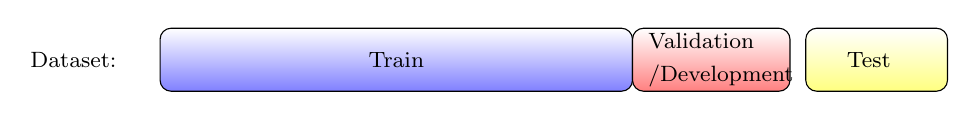
\begin{tikzpicture}
[split/.style={rectangle,rounded corners,draw=black, top color=white, bottom color=blue!50, thin, inner sep=0.25em, minimum size=0.1em, text centered}]
\draw[split] (0,0.1) rectangle (6,0.9); 
\draw[split,bottom color=red!50] (6,0.1) rectangle (8,0.9); 
\draw[split,bottom color=yellow!50] (8.2,0.1) rectangle (10,0.9); 

\node[draw=none,inner sep=1pt]  at (-1.1,0.5) {\footnotesize Dataset:}; 
\node[draw=none,inner sep=1pt]  at (3,0.5) {\footnotesize Train};  
\node[draw=none,inner sep=1pt,text width=1cm]  at (6.7,0.5) {\footnotesize Validation\newline 
/Development}; 
\node[draw=none,inner sep=1pt]  at (9,0.5) {\footnotesize Test};
\end{tikzpicture}
\begin{itemize}
\item Train a set of models $H$ with different hyperparameters
\item Choose the model $h$ that maximises performance on a validation set.
	\begin{itemize}
	\item Can't  tune on the training set as it would lead to overfitting %where the model cannot generalise to new data points in the test set.
\end{itemize}
\uncover<2->{\item Strength: optimises a performance metric we really care about.}
\uncover<3->{\item Weakness: we didn't use all the data in training; }
\uncover<4->{\item Weakness: if the validation set is small, we might choose the wrong model!}
\end{itemize}

\end{frame}


\begin{frame}
\frametitle{Model Selection on a Validation Set}
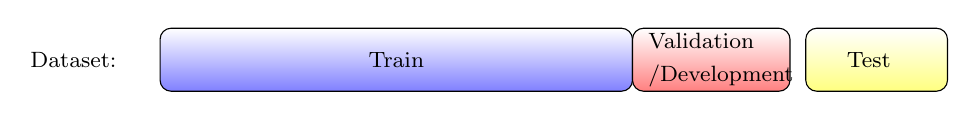
\begin{tikzpicture}
[split/.style={rectangle,rounded corners,draw=black, top color=white, bottom color=blue!50, thin, inner sep=0.25em, minimum size=0.1em, text centered}]
\draw[split] (0,0.1) rectangle (6,0.9); 
\draw[split,bottom color=red!50] (6,0.1) rectangle (8,0.9); 
\draw[split,bottom color=yellow!50] (8.2,0.1) rectangle (10,0.9); 

\node[draw=none,inner sep=1pt]  at (-1.1,0.5) {\footnotesize Dataset:}; 
\node[draw=none,inner sep=1pt]  at (3,0.5) {\footnotesize Train};  
\node[draw=none,inner sep=1pt,text width=1cm]  at (6.7,0.5) {\footnotesize Validation\newline 
/Development}; 
\node[draw=none,inner sep=1pt]  at (9,0.5) {\footnotesize Test};
\end{tikzpicture}
\begin{itemize}
\item Train a set of models $H$ with different hyperparameters
\item Choose the model $h$ that maximises performance on a validation set.
\uncover<2->{\item How do we come up with $H$?}
\uncover<3->{\item Random search: test random combinations of hyperparameters}
\uncover<4->{\item Grid search: For each hyperparameter,  define a set of values to test
	\begin{itemize}
		\item Use your knowledge of the problem to test only reasonable values
		\item For numerical hyperparameters,  e.g., learning rate, choose a set of evenly-spaced values within a sensible range
		\item $H$ contains all combinations of the chosen hyperparameter values
	\end{itemize}}
\uncover<5->{\item Reduce the number of tests needed to find a good combination using a more intelligent strategy such as Bayesian Optimisation}
\end{itemize}

\end{frame}


\begin{frame}
\frametitle{Cross-validation}
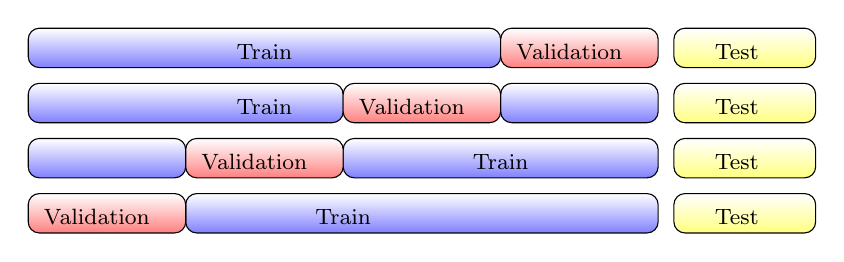
\begin{tikzpicture}
[split/.style={rectangle,rounded corners,draw=black, top color=white, bottom color=blue!50, thin, inner sep=0.25em, minimum size=0.1em, text centered}]
\draw[split] (0,2.2) rectangle (6,2.7); 
\draw[split,bottom color=red!50] (6,2.2) rectangle (8,2.7); 
\draw[split,bottom color=yellow!50] (8.2,2.2) rectangle (10,2.7); 

\node[draw=none,inner sep=1pt]  at (3,2.4) {\footnotesize Train};  
\node[draw=none,inner sep=1pt,text width=1cm]  at (6.7,2.4) {\footnotesize Validation}; 
\node[draw=none,inner sep=1pt]  at (9,2.4) {\footnotesize Test};

% second row
\draw[split] (0,1.5) rectangle (4,2); 
\draw[split] (6,1.5) rectangle (8,2); 
\draw[split,bottom color=red!50] (4,1.5) rectangle (6,2); 
\draw[split,bottom color=yellow!50] (8.2,1.5) rectangle (10,2); 

\node[draw=none,inner sep=1pt]  at (3,1.7) {\footnotesize Train};  
\node[draw=none,inner sep=1pt,text width=1cm]  at (4.7,1.7) {\footnotesize Validation}; 
\node[draw=none,inner sep=1pt]  at (9,1.7) {\footnotesize Test};

% third row
\draw[split] (0,0.8) rectangle (2,1.3); 
\draw[split] (4,0.8) rectangle (8,1.3); 
\draw[split,bottom color=red!50] (2,0.8) rectangle (4,1.3); 
\draw[split,bottom color=yellow!50] (8.2,0.8) rectangle (10,1.3); 

\node[draw=none,inner sep=1pt]  at (6,1) {\footnotesize Train};  
\node[draw=none,inner sep=1pt,text width=1cm]  at (2.7,1) {\footnotesize Validation}; 
\node[draw=none,inner sep=1pt]  at (9,1) {\footnotesize Test};

% fourth row
\draw[split] (2,0.1) rectangle (8,0.6); 
\draw[split,bottom color=red!50] (0,0.1) rectangle (2,0.6); 
\draw[split,bottom color=yellow!50] (8.2,0.1) rectangle (10,0.6); 

\node[draw=none,inner sep=1pt]  at (4,0.3) {\footnotesize Train};  
\node[draw=none,inner sep=1pt,text width=1cm]  at (0.7,0.3) {\footnotesize Validation}; 
\node[draw=none,inner sep=1pt]  at (9,0.3) {\footnotesize Test};

\end{tikzpicture}
\begin{itemize}
\item Split the training data into $k$ random, equally-sized subsets;
\item For each of the $k$ folds: leave out the $k$th subset from training, train on the rest and test on the $k$th subset;
\item Compute the average performance across all $k$ folds;
\item Avoids overfitting by tuning on training set performance...
\item And avoids tuning on a single small validation set.
\end{itemize}

\end{frame}

\begin{frame}[fragile]
\frametitle{Agenda}   % expectation: 33 slides + title and agenda, 11 slides per chunk
\begin{itemize}
\item \textcolor{gray}{Model Selection}
\item Model Averaging
\item Ensembles: Bagging
\item Ensembles: Boosting and Stacking
\item \textcolor{gray}{Tree-based Models  
\item Conditional Mixture Models 
\item Ensembles of Humans} 
\end{itemize}
\end{frame}

% keep this order because (a) it follows the book and 
%(b) committees often follow the same principle as model averaging
%but are usually unweighted.


\begin{frame}
\frametitle{Bayesian Model Averaging (BMA)}

\begin{itemize}
\item Model selection does not always pick out one model,  $h$,  as a clear winner 
\item We may be \emph{uncertain} about which model is correct
\uncover<2->{\item We can express uncertainty by assigning a probability to each model given 
the training data, $p(h|\bs X)$.}
\end{itemize}

\end{frame}


\begin{frame}
\frametitle{Bayesian Model Averaging (BMA)}

\begin{itemize}
\item Rather than choosing a single model, we can now take an expectation.
\item Our predictions now come from a \emph{weighted sum} over models, where $p(h|\bs X)$ are weights :
\end{itemize}

\begin{equation}
p(\bs z | \bs X) = \sum_{h=1}^H p(\bs z | \bs X, h)p(h|\bs X)
\end{equation}

\end{frame}


\begin{frame}
\frametitle{Bayesian Model Averaging (BMA)}
\begin{itemize}
\item Apply Bayes' rule to estimate the weights:
\end{itemize}

\begin{equation}
p(h|\bs X) = \frac{p(\bs X | h)p(h)}{\sum_{h'=1}^H p(\bs X | h')p(h')}
\end{equation}

\begin{itemize}
\item What happens as we increase the amount of data in $\bs X$?
\uncover<2->{\item $p(h|\bs X)$ becomes more focussed on one model.
\item So BMA is soft model selection, it does not \emph{combine} models to make a more powerful model.}
%It is a way to handle uncertainty about which model is correct, not to combine the strengths of multiple models.
% it doesn't outperform the individual models in expectation, whereas combination effectively creates a new model
\end{itemize}
\end{frame}


\begin{frame}
\frametitle{Ensemble Methods}
\begin{itemize}
\item \textcolor{gray}{Model Selection
\item Model Averaging}
\item Ensembles: Bagging
\item Ensembles: Boosting and Stacking
\item \textcolor{gray}{Tree-based Models  
\item Conditional Mixture Models 
\item Ensembles of Humans} 
\end{itemize}
\end{frame}

\begin{frame}
\frametitle{Wisdom of the crowd}
Guess the weight!

\uncover<2->{In 1907, Sir Francis Galton asked 787 villagers to guess the weight of an ox. 
None of them got the right answer,  but when Galton averaged their guesses,  
he arrived at a near perfect estimate.}

\uncover<3->{\textbf{The combination was more effective than any one `model'.}}

\centering
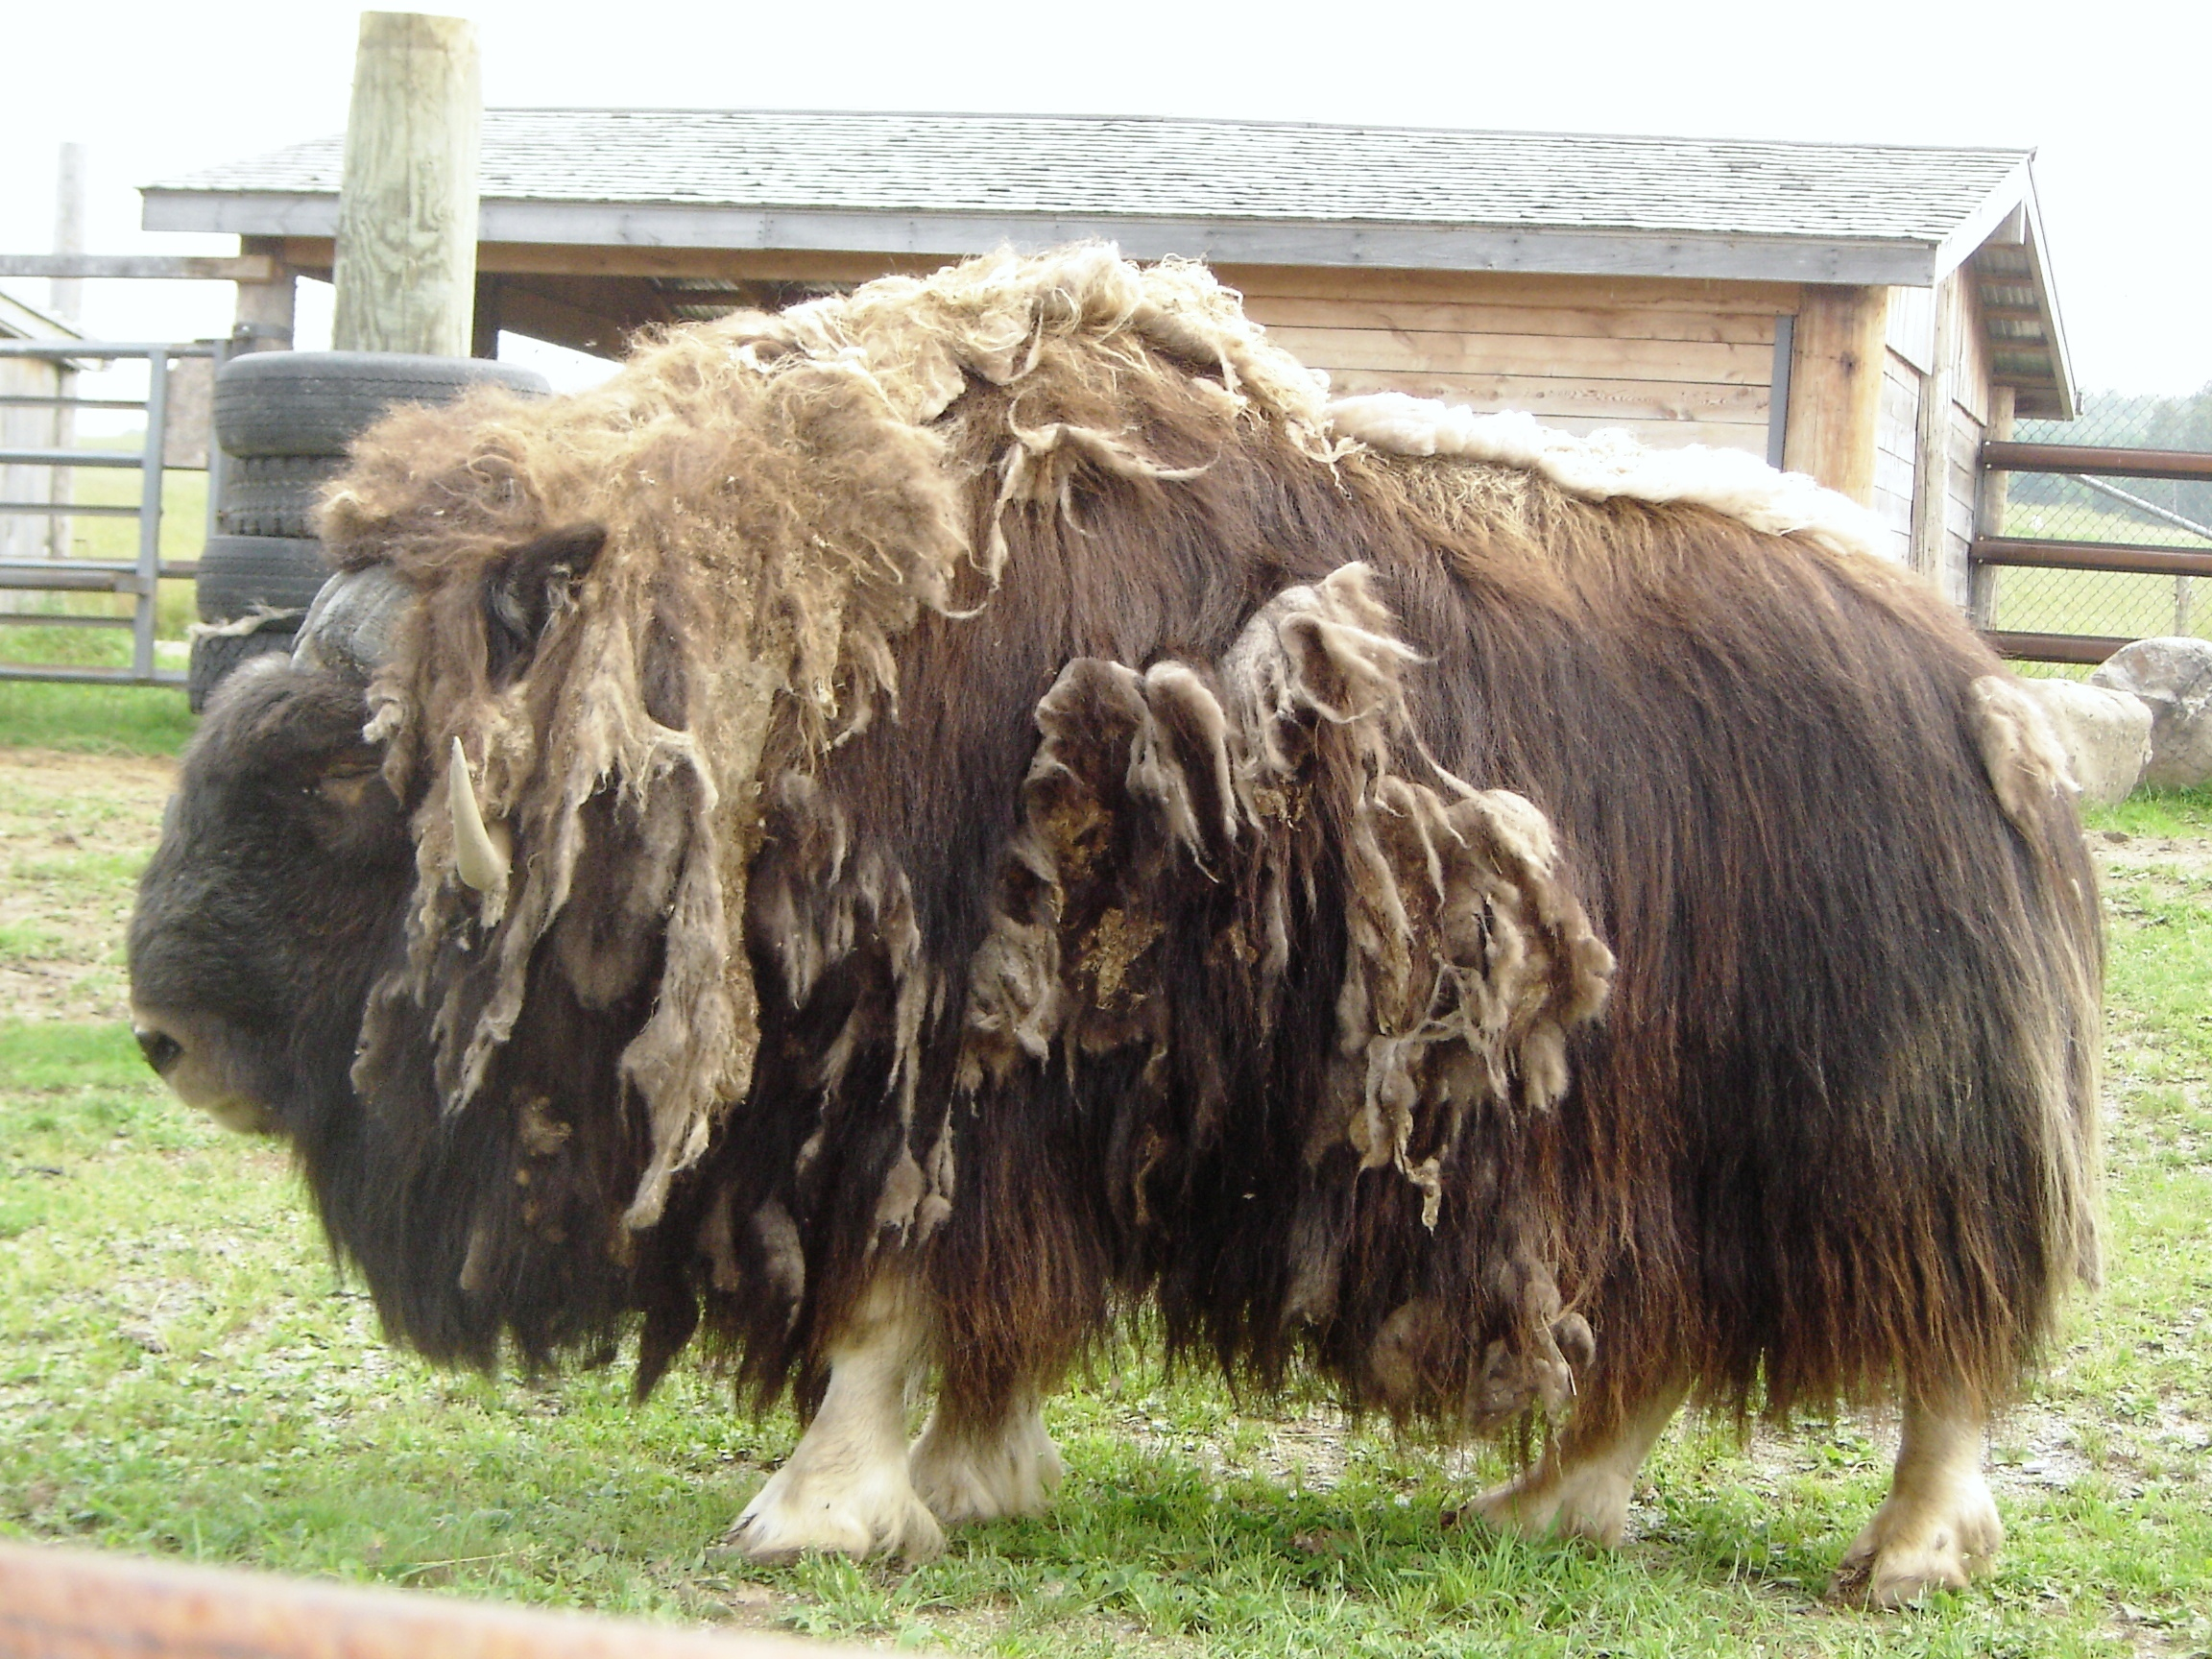
\includegraphics[scale=0.07]{../figures/Musk_ox}
\end{frame}

\begin{frame}
\frametitle{Ensemble Methods}
\begin{itemize}
\item Ensemble: a combination of different models.
\item Often outperforms the average individual, and sometimes even the best individual.
\item Different principle to BMA: 
\begin{itemize}
\item BMA weights try to identify a single, correct model
\item BMA weights do not provide the optimal combination
\end{itemize}
%\item Difference to mixture of experts or decision trees: we don't split the input space between models, multiple models are combined for each data point.
\end{itemize}
\end{frame}


% why does it outperform? look at the errors in the simple case
\begin{frame}
\frametitle{Expected Error of an Ensemble}

\begin{itemize}
\item  Given a set of models, $1,...,M$,
\item $y_m(\bs x)$ is the prediction from model $m$.
\item Simple ensemble: the mean of the individual predictions,
$y_{COM} = \frac{1}{M} \sum_{m=1}^M y_m(\bs x)$,
\uncover<2->{\item Let's compare the sum-of-squares error of $y_{COM}$ with that of the individual models...}
\end{itemize}

\end{frame}

\begin{frame}
\frametitle{Expected Error of an Ensemble}

Firstly, the error of our combination for a particular input $\bs x$ is:
\begin{equation}
(y(\bs x) - y_{COM}(\bs x))^2 = \left(\frac{1}{M}\sum_{m=1}^M \left( y(\bs x) - y_m(\bs x)\right)\right)^2.
\end{equation}
\end{frame}

\begin{frame}
\frametitle{Expected Error of an Ensemble}

Firstly, the expected error of our combination is:
\begin{equation}
E_{COM} = 
\mathbb{E}_{\bs x}[(y(\bs x) - y_{COM}(\bs x))^2] = \mathbb{E}_{\bs x}\left[\left(\frac{1}{M}\sum_{m=1}^M (y(\bs x) - y_m(\bs x))\right)^2\right].
\end{equation}
\end{frame}

\begin{frame}
\frametitle{Expected Error of an Ensemble}

\begin{itemize}
\item The expected error of an individual model $m$ is: 
 $E_{m} =  \mathbb{E}_{\bs x}[ (y(\bs x) - y_m(\bs x))^2]$.
\end{itemize}

\end{frame}


\begin{frame}
\frametitle{Expected Error of an Ensemble}

\begin{itemize}
\item The \textbf{average} expected error of an individual model is: 
 $E_{AV} = \frac{1}{M} \sum_{m=1}^M \mathbb{E}_{\bs x}\left[ (y(\bs x) - y_m(\bs x))^2\right]$.
\uncover<2->{\item Remember: $E_{COM} = \mathbb{E}_{\bs x}\left[\left(\frac{1}{M}\sum_{m=1}^M (y(\bs x) - y_m(\bs x))\right)^2\right]$.}
\uncover<3->{\item ...so we have $E_{COM} = \frac{1}{M} E_{AV}$, since for $E_{COM}$, the $\frac{1}{M}$ is squared}
\uncover<4->{\item This relies on two assumptions...
	\begin{enumerate}
	\item The errors of each model have zero mean;
	\item The errors of different models are not correlated;
	\end{enumerate}}
\uncover<5->{\item Intuition: if models make different, random errors, they will tend to cancel out.}
\end{itemize}

\end{frame}


\begin{frame}
\frametitle{Expected Error of an Ensemble}

\begin{itemize}
\item $E_{COM} = \frac{1}{M} E_{AV}$ is pretty amazing, but is it realistic?
\uncover<2->{\item No, because we have made extreme assumptions about the models' errors -- in practice, they are usually highly correlated and biased.}
\uncover<3->{\item However, the combined error cannot be worse than the average error:$E_{COM} \leq E_{AV}$\footnote{This bound is due to \emph{Jensen's inequality}.}
% the assumptions also tell us about what to aim for when designing the ensemble.
\item The results tells us that the models should be \emph{diverse} 
to avoid repeating the same errors.}
\end{itemize}

\end{frame}

% Ensemble methods are about desigining base models that maximise diversity of errors.
\begin{frame}
\frametitle{Bootstrap Aggregation (Bagging)}
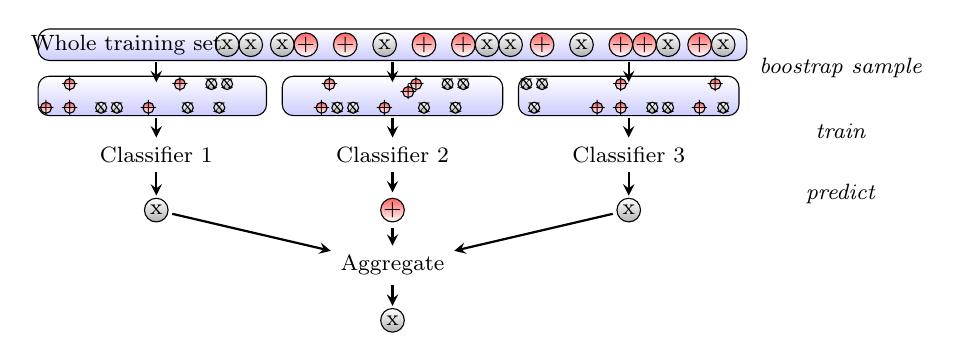
\begin{tikzpicture}
[split/.style={rectangle,rounded corners,draw=black, top color=white, bottom color=blue!20, thin, inner sep=0.25em, minimum size=0.1em, text centered},
classical/.style={thick,->,shorten >=0pt,shorten <=0pt,>=stealth},
flow/.style={thick, gray, decoration={markings,mark=at position
   1 with {\arrow[thick,gray]{ triangle 60}}},
   double distance=6.5pt, shorten >= 6.5pt,
   preaction = {decorate, gray},
   postaction = {draw,line width=7pt, gray,shorten >= 6.3pt}},]
\draw[split] (0,2.2) rectangle (9,2.6); 
\node[draw=none] (1s) at (1.5,2.3){};
\node[draw=none] (2s) at (4.5,2.3){};
\node[draw=none] (3s) at (7.5,2.3){};

\draw[top color=white, bottom color=gray!60](5.7,2.4) circle (0.15cm);
\node[draw=none] at (5.7,2.4) {\footnotesize x};
\draw[top color=red!60](7.7,2.4) circle (0.15cm);
\node[draw=none] at (7.7,2.4) {\footnotesize +};

\draw[top color=white, bottom color=gray!60](2.7,2.4) circle (0.15cm);
\node[draw=none] at (2.7,2.4) {\footnotesize x};
\draw[top color=red!60](3.4,2.4) circle (0.15cm);
\node[draw=none] at (3.4,2.4) {\footnotesize +};

\draw[top color=white, bottom color=gray!60](2.4,2.4) circle (0.15cm);
\node[draw=none] at (2.4,2.4) {\footnotesize x};
\draw[top color=red!60](3.9,2.4) circle (0.15cm);
\node[draw=none] at (3.9,2.4) {\footnotesize +};

\draw[top color=white, bottom color=gray!60](3.1,2.4) circle (0.15cm);
\node[draw=none] at (3.1,2.4) {\footnotesize x};
\draw[top color=red!60](5.4,2.4) circle (0.15cm);
\node[draw=none] at (5.4,2.4) {\footnotesize +};

\draw[top color=white, bottom color=gray!60](4.4,2.4) circle (0.15cm);
\node[draw=none] at (4.4,2.4) {\footnotesize x};
\draw[top color=red!60](4.9,2.4) circle (0.15cm);
\node[draw=none] at (4.9,2.4) {\footnotesize +};

\draw[top color=white, bottom color=gray!60](6,2.4) circle (0.15cm);
\node[draw=none] at (6,2.4) {\footnotesize x};
\draw[top color=red!60](6.4,2.4) circle (0.15cm);
\node[draw=none] at (6.4,2.4) {\footnotesize +};

\draw[top color=white, bottom color=gray!60](6.9,2.4) circle (0.15cm);
\node[draw=none] at (6.9,2.4) {\footnotesize x};
\draw[top color=red!60](7.4,2.4) circle (0.15cm);
\node[draw=none] at (7.4,2.4) {\footnotesize +};

\draw[top color=white, bottom color=gray!60](8,2.4) circle (0.15cm);
\node[draw=none] at (8,2.4) {\footnotesize x};
\draw[top color=red!60](8.4,2.4) circle (0.15cm);
\node[draw=none] at (8.4,2.4) {\footnotesize +};

\draw[top color=white, bottom color=gray!60](8.7,2.4) circle (0.15cm);
\node[draw=none] at (8.7,2.4) {\footnotesize x};

\node[draw=none,inner sep=1pt]  at (1.12,2.4) {\footnotesize Whole training set};  

% second row
\draw[split] (0,1.5) rectangle (2.9,2); 
\draw[split] (3.1,1.5) rectangle (5.9,2); 
\draw[split] (6.1,1.5) rectangle (8.9,2); 

\node[draw=none] (1) at (1.5,1.8){};
\node[draw=none] (2) at (4.5,1.8){};
\node[draw=none] (3) at (7.5,1.8){};

\draw[classical] (1s) to (1);
\draw[classical] (2s) to (2);
\draw[classical] (3s) to (3);

\node[draw=none,inner sep=1pt]  (tv) at (10.2,2.1) {\footnotesize \textit{boostrap sample}};

\draw[top color=white, bottom color=gray!60](1,1.6) circle (0.07cm);
\node[draw=none] at (1,1.6) {\footnotesize x};
\draw[top color=red!60](1.4,1.6) circle (0.07);
\node[draw=none] at (1.4,1.6) {\footnotesize +};
\draw[top color=white, bottom color=gray!60](1.9,1.6) circle (0.07);
\node[draw=none] at (1.9,1.6) {\footnotesize x};
\draw[top color=red!60](0.4,1.6) circle (0.07);
\node[draw=none] at (0.4,1.6) {\footnotesize +};
\draw[top color=white, bottom color=gray!60](0.8,1.6) circle (0.07);
\node[draw=none] at (0.8,1.6) {\footnotesize x};
\draw[top color=red!60](0.1,1.6) circle (0.07);
\node[draw=none] at (0.1,1.6) {\footnotesize +};
\draw[top color=white, bottom color=gray!60](2.3,1.6) circle (0.07);
\node[draw=none] at (2.3,1.6) {\footnotesize x};
\draw[top color=red!60](0.4,1.9) circle (0.07);
\node[draw=none] at (0.4,1.9) {\footnotesize +};
\draw[top color=white, bottom color=gray!60](2.4,1.9) circle (0.07);
\node[draw=none] at (2.4,1.9) {\footnotesize x};
\draw[top color=red!60](1.8,1.9) circle (0.07);
\node[draw=none] at (1.8,1.9) {\footnotesize +};
\draw[top color=white, bottom color=gray!60](2.2,1.9) circle (0.07);
\node[draw=none] at (2.2,1.9) {\footnotesize x};

\draw[top color=white, bottom color=gray!60](4,1.6) circle (0.07cm);
\node[draw=none] at (4,1.6) {\footnotesize x};
\draw[top color=red!60](4.4,1.6) circle (0.07);
\node[draw=none] at (4.4,1.6) {\footnotesize +};
\draw[top color=white, bottom color=gray!60](4.9,1.6) circle (0.07);
\node[draw=none] at (4.9,1.6) {\footnotesize x};
\draw[top color=red!60](4.7,1.8) circle (0.07);
\node[draw=none] at (4.7,1.8) {\footnotesize +};
\draw[top color=white, bottom color=gray!60](3.8,1.6) circle (0.07);
\node[draw=none] at (3.8,1.6) {\footnotesize x};
\draw[top color=red!60](3.6,1.6) circle (0.07);
\node[draw=none] at (3.6,1.6) {\footnotesize +};
\draw[top color=white, bottom color=gray!60](5.3,1.6) circle (0.07);
\node[draw=none] at (5.3,1.6) {\footnotesize x};
\draw[top color=red!60](3.7,1.9) circle (0.07);
\node[draw=none] at (3.7,1.9) {\footnotesize +};
\draw[top color=white, bottom color=gray!60](5.4,1.9) circle (0.07);
\node[draw=none] at (5.4,1.9) {\footnotesize x};
\draw[top color=red!60](4.8,1.9) circle (0.07);
\node[draw=none] at (4.8,1.9) {\footnotesize +};
\draw[top color=white, bottom color=gray!60](5.2,1.9) circle (0.07);
\node[draw=none] at (5.2,1.9) {\footnotesize x};

\draw[top color=white, bottom color=gray!60](8,1.6) circle (0.07cm);
\node[draw=none] at (8,1.6) {\footnotesize x};
\draw[top color=red!60](8.4,1.6) circle (0.07);
\node[draw=none] at (8.4,1.6) {\footnotesize +};
\draw[top color=white, bottom color=gray!60](8.7,1.6) circle (0.07);
\node[draw=none] at (8.7,1.6) {\footnotesize x};
\draw[top color=red!60](7.4,1.6) circle (0.07);
\node[draw=none] at (7.4,1.6) {\footnotesize +};
\draw[top color=white, bottom color=gray!60](7.8,1.6) circle (0.07);
\node[draw=none] at (7.8,1.6) {\footnotesize x};
\draw[top color=red!60](7.1,1.6) circle (0.07);
\node[draw=none] at (7.1,1.6) {\footnotesize +};
\draw[top color=white, bottom color=gray!60](6.3,1.6) circle (0.07);
\node[draw=none] at (6.3,1.6) {\footnotesize x};
\draw[top color=red!60](7.4,1.9) circle (0.07);
\node[draw=none] at (7.4,1.9) {\footnotesize +};
\draw[top color=white, bottom color=gray!60](6.4,1.9) circle (0.07);
\node[draw=none] at (6.4,1.9) {\footnotesize x};
\draw[top color=red!60](8.6,1.9) circle (0.07);
\node[draw=none] at (8.6,1.9) {\footnotesize +};
\draw[top color=white, bottom color=gray!60](6.2,1.9) circle (0.07);
\node[draw=none] at (6.2,1.9) {\footnotesize x};

% third row
%\draw[split,bottom color=yellow!50] (9.2,1.1) rectangle (11.2,1.6); 
%\node[draw=none,inner sep=1pt]  (tv) at (10.2,1.3) {\footnotesize Test/Validation};

\node[draw=none,inner sep=1pt]  (tv) at (10.2,1.3) {\footnotesize \textit{train}};

\node[draw=none] (1cs) at (1.5,1.6){ };
\node[draw=none] (2cs) at (4.5,1.6){};
\node[draw=none] (3cs) at (7.5,1.6){};

\node[draw=none] (1c) at (1.5,1){\footnotesize Classifier 1};
\node[draw=none] (2c) at (4.5,1){\footnotesize Classifier 2};
\node[draw=none] (3c) at (7.5,1){\footnotesize Classifier 3};

\draw[classical] (1cs) to (1c);
\draw[classical] (2cs) to (2c);
\draw[classical] (3cs) to (3c);

%\draw[classical] (tv) to (3c);
%\draw[classical] (tv) to (2c);
%\draw[classical] (tv) to (1c);


% fourth row
\node[draw=none,inner sep=1pt]  (tv) at (10.2,0.5) {\footnotesize \textit{predict}};

\draw[top color=white, bottom color=gray!60](1.5,0.3) circle (0.15);
\node[draw=none] (1p) at (1.5,0.3) {\footnotesize x};
\draw[top color=red!60](4.5,0.3) circle (0.15);
\node[draw=none] (2p) at (4.5,0.3) {\footnotesize +};
\draw[top color=white, bottom color=gray!60](7.5,0.3) circle (0.15);
\node[draw=none] (3p) at (7.5,0.3) {\footnotesize x};


\draw[classical] (1c) to (1p);
\draw[classical] (2c) to (2p);
\draw[classical] (3c) to (3p);

% fifth row
\node[draw=none] (a) at (4.5,-0.4) {\footnotesize Aggregate};

\draw[top color=white, bottom color=gray!60](4.5,-1.1) circle (0.15);
\node[draw=none] (ap) at (4.5,-1.1) {\footnotesize x};

\draw[classical] (1p) to (a);
\draw[classical] (2p) to (a);
\draw[classical] (3p) to (a);

\draw[classical] (a) to (ap);

%\draw[split] (2,0.1) rectangle (8,0.6); 
%\draw[split,bottom color=red!50] (0,0.1) rectangle (2,0.6); 
%\draw[split,bottom color=yellow!50] (8.2,0.1) rectangle (10,0.6); 
%
%\node[draw=none,inner sep=1pt]  at (4,0.3) {\footnotesize Train};  
%\node[draw=none,inner sep=1pt,text width=1cm]  at (0.7,0.3) {\footnotesize Validation}; 
%\node[draw=none,inner sep=1pt]  at (9,0.3) {\footnotesize Test};

\end{tikzpicture}
\begin{itemize}
\item Create diversity by training models on different samples of the training set. 
\end{itemize}

\end{frame}

\begin{frame}
\frametitle{Bootstrap Aggregation (Bagging)}
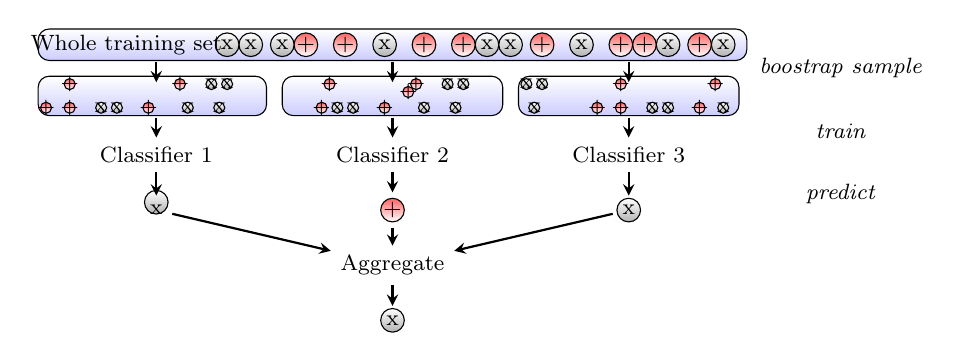
\begin{tikzpicture}
[split/.style={rectangle,rounded corners,draw=black, top color=white, bottom color=blue!20, thin, inner sep=0.25em, minimum size=0.1em, text centered},
classical/.style={thick,->,shorten >=0pt,shorten <=0pt,>=stealth},
flow/.style={thick, gray, decoration={markings,mark=at position
   1 with {\arrow[thick,gray]{ triangle 60}}},
   double distance=6.5pt, shorten >= 6.5pt,
   preaction = {decorate, gray},
   postaction = {draw,line width=7pt, gray,shorten >= 6.3pt}},]
\draw[split] (0,2.2) rectangle (9,2.6); 
\node[draw=none] (1s) at (1.5,2.3){};
\node[draw=none] (2s) at (4.5,2.3){};
\node[draw=none] (3s) at (7.5,2.3){};

\draw[top color=white, bottom color=gray!60](5.7,2.4) circle (0.15cm);
\node[draw=none] at (5.7,2.4) {\footnotesize x};
\draw[top color=red!60](7.7,2.4) circle (0.15cm);
\node[draw=none] at (7.7,2.4) {\footnotesize +};

\draw[top color=white, bottom color=gray!60](2.7,2.4) circle (0.15cm);
\node[draw=none] at (2.7,2.4) {\footnotesize x};
\draw[top color=red!60](3.4,2.4) circle (0.15cm);
\node[draw=none] at (3.4,2.4) {\footnotesize +};

\draw[top color=white, bottom color=gray!60](2.4,2.4) circle (0.15cm);
\node[draw=none] at (2.4,2.4) {\footnotesize x};
\draw[top color=red!60](3.9,2.4) circle (0.15cm);
\node[draw=none] at (3.9,2.4) {\footnotesize +};

\draw[top color=white, bottom color=gray!60](3.1,2.4) circle (0.15cm);
\node[draw=none] at (3.1,2.4) {\footnotesize x};
\draw[top color=red!60](5.4,2.4) circle (0.15cm);
\node[draw=none] at (5.4,2.4) {\footnotesize +};

\draw[top color=white, bottom color=gray!60](4.4,2.4) circle (0.15cm);
\node[draw=none] at (4.4,2.4) {\footnotesize x};
\draw[top color=red!60](4.9,2.4) circle (0.15cm);
\node[draw=none] at (4.9,2.4) {\footnotesize +};

\draw[top color=white, bottom color=gray!60](6,2.4) circle (0.15cm);
\node[draw=none] at (6,2.4) {\footnotesize x};
\draw[top color=red!60](6.4,2.4) circle (0.15cm);
\node[draw=none] at (6.4,2.4) {\footnotesize +};

\draw[top color=white, bottom color=gray!60](6.9,2.4) circle (0.15cm);
\node[draw=none] at (6.9,2.4) {\footnotesize x};
\draw[top color=red!60](7.4,2.4) circle (0.15cm);
\node[draw=none] at (7.4,2.4) {\footnotesize +};

\draw[top color=white, bottom color=gray!60](8,2.4) circle (0.15cm);
\node[draw=none] at (8,2.4) {\footnotesize x};
\draw[top color=red!60](8.4,2.4) circle (0.15cm);
\node[draw=none] at (8.4,2.4) {\footnotesize +};

\draw[top color=white, bottom color=gray!60](8.7,2.4) circle (0.15cm);
\node[draw=none] at (8.7,2.4) {\footnotesize x};

\node[draw=none,inner sep=1pt]  at (1.12,2.4) {\footnotesize Whole training set};  

% second row
\draw[split] (0,1.5) rectangle (2.9,2); 
\draw[split] (3.1,1.5) rectangle (5.9,2); 
\draw[split] (6.1,1.5) rectangle (8.9,2); 

\node[draw=none] (1) at (1.5,1.8){};
\node[draw=none] (2) at (4.5,1.8){};
\node[draw=none] (3) at (7.5,1.8){};

\draw[classical] (1s) to (1);
\draw[classical] (2s) to (2);
\draw[classical] (3s) to (3);

\node[draw=none,inner sep=1pt]  (tv) at (10.2,2.1) {\footnotesize \textit{boostrap sample}};

\draw[top color=white, bottom color=gray!60](1,1.6) circle (0.07cm);
\node[draw=none] at (1,1.6) {\footnotesize x};
\draw[top color=red!60](1.4,1.6) circle (0.07);
\node[draw=none] at (1.4,1.6) {\footnotesize +};
\draw[top color=white, bottom color=gray!60](1.9,1.6) circle (0.07);
\node[draw=none] at (1.9,1.6) {\footnotesize x};
\draw[top color=red!60](0.4,1.6) circle (0.07);
\node[draw=none] at (0.4,1.6) {\footnotesize +};
\draw[top color=white, bottom color=gray!60](0.8,1.6) circle (0.07);
\node[draw=none] at (0.8,1.6) {\footnotesize x};
\draw[top color=red!60](0.1,1.6) circle (0.07);
\node[draw=none] at (0.1,1.6) {\footnotesize +};
\draw[top color=white, bottom color=gray!60](2.3,1.6) circle (0.07);
\node[draw=none] at (2.3,1.6) {\footnotesize x};
\draw[top color=red!60](0.4,1.9) circle (0.07);
\node[draw=none] at (0.4,1.9) {\footnotesize +};
\draw[top color=white, bottom color=gray!60](2.4,1.9) circle (0.07);
\node[draw=none] at (2.4,1.9) {\footnotesize x};
\draw[top color=red!60](1.8,1.9) circle (0.07);
\node[draw=none] at (1.8,1.9) {\footnotesize +};
\draw[top color=white, bottom color=gray!60](2.2,1.9) circle (0.07);
\node[draw=none] at (2.2,1.9) {\footnotesize x};

\draw[top color=white, bottom color=gray!60](4,1.6) circle (0.07cm);
\node[draw=none] at (4,1.6) {\footnotesize x};
\draw[top color=red!60](4.4,1.6) circle (0.07);
\node[draw=none] at (4.4,1.6) {\footnotesize +};
\draw[top color=white, bottom color=gray!60](4.9,1.6) circle (0.07);
\node[draw=none] at (4.9,1.6) {\footnotesize x};
\draw[top color=red!60](4.7,1.8) circle (0.07);
\node[draw=none] at (4.7,1.8) {\footnotesize +};
\draw[top color=white, bottom color=gray!60](3.8,1.6) circle (0.07);
\node[draw=none] at (3.8,1.6) {\footnotesize x};
\draw[top color=red!60](3.6,1.6) circle (0.07);
\node[draw=none] at (3.6,1.6) {\footnotesize +};
\draw[top color=white, bottom color=gray!60](5.3,1.6) circle (0.07);
\node[draw=none] at (5.3,1.6) {\footnotesize x};
\draw[top color=red!60](3.7,1.9) circle (0.07);
\node[draw=none] at (3.7,1.9) {\footnotesize +};
\draw[top color=white, bottom color=gray!60](5.4,1.9) circle (0.07);
\node[draw=none] at (5.4,1.9) {\footnotesize x};
\draw[top color=red!60](4.8,1.9) circle (0.07);
\node[draw=none] at (4.8,1.9) {\footnotesize +};
\draw[top color=white, bottom color=gray!60](5.2,1.9) circle (0.07);
\node[draw=none] at (5.2,1.9) {\footnotesize x};

\draw[top color=white, bottom color=gray!60](8,1.6) circle (0.07cm);
\node[draw=none] at (8,1.6) {\footnotesize x};
\draw[top color=red!60](8.4,1.6) circle (0.07);
\node[draw=none] at (8.4,1.6) {\footnotesize +};
\draw[top color=white, bottom color=gray!60](8.7,1.6) circle (0.07);
\node[draw=none] at (8.7,1.6) {\footnotesize x};
\draw[top color=red!60](7.4,1.6) circle (0.07);
\node[draw=none] at (7.4,1.6) {\footnotesize +};
\draw[top color=white, bottom color=gray!60](7.8,1.6) circle (0.07);
\node[draw=none] at (7.8,1.6) {\footnotesize x};
\draw[top color=red!60](7.1,1.6) circle (0.07);
\node[draw=none] at (7.1,1.6) {\footnotesize +};
\draw[top color=white, bottom color=gray!60](6.3,1.6) circle (0.07);
\node[draw=none] at (6.3,1.6) {\footnotesize x};
\draw[top color=red!60](7.4,1.9) circle (0.07);
\node[draw=none] at (7.4,1.9) {\footnotesize +};
\draw[top color=white, bottom color=gray!60](6.4,1.9) circle (0.07);
\node[draw=none] at (6.4,1.9) {\footnotesize x};
\draw[top color=red!60](8.6,1.9) circle (0.07);
\node[draw=none] at (8.6,1.9) {\footnotesize +};
\draw[top color=white, bottom color=gray!60](6.2,1.9) circle (0.07);
\node[draw=none] at (6.2,1.9) {\footnotesize x};

% third row
%\draw[split,bottom color=yellow!50] (9.2,1.1) rectangle (11.2,1.6); 
%\node[draw=none,inner sep=1pt]  (tv) at (10.2,1.3) {\footnotesize Test/Validation};

\node[draw=none,inner sep=1pt]  (tv) at (10.2,1.3) {\footnotesize \textit{train}};

\node[draw=none] (1cs) at (1.5,1.6){ };
\node[draw=none] (2cs) at (4.5,1.6){};
\node[draw=none] (3cs) at (7.5,1.6){};

\node[draw=none] (1c) at (1.5,1){\footnotesize Classifier 1};
\node[draw=none] (2c) at (4.5,1){\footnotesize Classifier 2};
\node[draw=none] (3c) at (7.5,1){\footnotesize Classifier 3};

\draw[classical] (1cs) to (1c);
\draw[classical] (2cs) to (2c);
\draw[classical] (3cs) to (3c);

%\draw[classical] (tv) to (3c);
%\draw[classical] (tv) to (2c);
%\draw[classical] (tv) to (1c);


% fourth row
\node[draw=none,inner sep=1pt]  (tv) at (10.2,0.5) {\footnotesize \textit{predict}};

\draw[top color=white, bottom color=gray!60](1.5,0.4) circle (0.15);
\node[draw=none] (1p) at (1.5,0.3) {\footnotesize x};
\draw[top color=red!60](4.5,0.3) circle (0.15);
\node[draw=none] (2p) at (4.5,0.3) {\footnotesize +};
\draw[top color=white, bottom color=gray!60](7.5,0.3) circle (0.15);
\node[draw=none] (3p) at (7.5,0.3) {\footnotesize x};


\draw[classical] (1c) to (1p);
\draw[classical] (2c) to (2p);
\draw[classical] (3c) to (3p);

% fifth row
\node[draw=none] (a) at (4.5,-0.4) {\footnotesize Aggregate};

\draw[top color=white, bottom color=gray!60](4.5,-1.1) circle (0.15);
\node[draw=none] (ap) at (4.5,-1.1) {\footnotesize x};

\draw[classical] (1p) to (a);
\draw[classical] (2p) to (a);
\draw[classical] (3p) to (a);

\draw[classical] (a) to (ap);

%\draw[split] (2,0.1) rectangle (8,0.6); 
%\draw[split,bottom color=red!50] (0,0.1) rectangle (2,0.6); 
%\draw[split,bottom color=yellow!50] (8.2,0.1) rectangle (10,0.6); 
%
%\node[draw=none,inner sep=1pt]  at (4,0.3) {\footnotesize Train};  
%\node[draw=none,inner sep=1pt,text width=1cm]  at (0.7,0.3) {\footnotesize Validation}; 
%\node[draw=none,inner sep=1pt]  at (9,0.3) {\footnotesize Test};

\end{tikzpicture}
\begin{itemize}
\item Create diversity by training models on different samples of the training set. 
\item For each model $m$, randomly sample $N$ data points with replacement from a training set with $N$ data points and train $m$ on the subsample.
\item In each sample, some data points will be repeated and others will be omitted. 
\item Combine predictions by taking the mean or majority vote.
\end{itemize}

\end{frame}

\begin{frame}
\frametitle{Boosting}

\begin{itemize}
\item Can we do better than choosing training sets at random?
\uncover<2->{\item Train \emph{base} models sequentially, ensuring that each base model addresses the weaknesses of the ensemble.
\item Instead of random sampling,  weight the data points in the training set according to the performance of previous base models.}
\uncover<3->{\item \emph{AdaBoost} is a popular boosting method originally designed for \emph{binary classification}.}
\end{itemize}

\end{frame}


\begin{frame}
\frametitle{AdaBoost}

Training sequence $\rightarrow$ \\
\raggedleft
\begin{overpic}[scale=0.4]{../figures/adaboost_diagram}
 \put (-43,50) {\framebox{\parbox{3cm}{train new classifier on weighted data that outputs class labels $+1$ or $-1$}}}
  \put(20,22){\setlength{\fboxsep}{4cm}\fcolorbox{white}{white}{}}

 \put(10,49){\setlength{\fboxsep}{0.74cm}\fcolorbox{white}{white}{}}
  \put(37,49){\setlength{\fboxsep}{0.74cm}\fcolorbox{white}{white}{}}
  \put(20,49){\setlength{\fboxsep}{0.74cm}\fcolorbox{white}{white}{}}
 \put(66,49){\setlength{\fboxsep}{0.74cm}\fcolorbox{white}{white}{}}
 \put(86,49){\setlength{\fboxsep}{0.74cm}\fcolorbox{white}{white}{}}

 \put(8,28){\setlength{\fboxsep}{0.6cm}\fcolorbox{white}{white}{}}
 \put(22,25){\setlength{\fboxsep}{0.87cm}\fcolorbox{white}{white}{}}
 \put(43,25){\setlength{\fboxsep}{0.74cm}\fcolorbox{white}{white}{}}
 \put(61,25){\setlength{\fboxsep}{0.74cm}\fcolorbox{white}{white}{}}
 \put(78,25){\setlength{\fboxsep}{0.74cm}\fcolorbox{white}{white}{}}

 %\put (-40,45) {compute weights from performance of previous model}
 %\put (-40,25) {after all models are trained, combine using a weighted sum}
\end{overpic}
\end{frame}

\begin{frame}
\frametitle{AdaBoost}

Training sequence $\rightarrow$ \\
\raggedleft
\begin{overpic}[scale=0.4]{../figures/adaboost_diagram}
 \put (-40,25) {\framebox{\parbox{3.2cm}{compute weights from performance of previous classifier}}}
   \put(20,22){\setlength{\fboxsep}{2cm}\fcolorbox{white}{white}{}}
   \put(44,22){\setlength{\fboxsep}{4cm}\fcolorbox{white}{white}{}}


 \put(-8,49){\setlength{\fboxsep}{0.74cm}\fcolorbox{white}{white}{}}
  \put(37,49){\setlength{\fboxsep}{0.74cm}\fcolorbox{white}{white}{}}
  \put(30,49){\setlength{\fboxsep}{0.74cm}\fcolorbox{white}{white}{}}
 \put(66,49){\setlength{\fboxsep}{0.74cm}\fcolorbox{white}{white}{}}
 \put(86,49){\setlength{\fboxsep}{0.74cm}\fcolorbox{white}{white}{}}

 \put(8,28){\setlength{\fboxsep}{0.6cm}\fcolorbox{white}{white}{}}
 \put(22,25){\setlength{\fboxsep}{0.87cm}\fcolorbox{white}{white}{}}
 \put(43,25){\setlength{\fboxsep}{0.74cm}\fcolorbox{white}{white}{}}
 \put(61,25){\setlength{\fboxsep}{0.74cm}\fcolorbox{white}{white}{}}
 \put(78,25){\setlength{\fboxsep}{0.74cm}\fcolorbox{white}{white}{}}
\end{overpic}
\end{frame}

\begin{frame}
\frametitle{AdaBoost}

Training sequence $\rightarrow$ \\
\raggedleft
\begin{overpic}[scale=0.4]{../figures/adaboost_diagram}
 \put (-40,25) {\framebox{\parbox{3.2cm}{compute weights from performance of previous classifier}}}
   \put(8,17){\setlength{\fboxsep}{1.45cm}\fcolorbox{white}{white}{}}
   \put(44,22){\setlength{\fboxsep}{4cm}\fcolorbox{white}{white}{}}


 \put(-8,49){\setlength{\fboxsep}{0.74cm}\fcolorbox{white}{white}{}}
  %\put(37,49){\setlength{\fboxsep}{0.74cm}\fcolorbox{white}{white}{}}
  \put(36,49){\setlength{\fboxsep}{0.74cm}\fcolorbox{white}{white}{}}
 %\put(66,49){\setlength{\fboxsep}{0.74cm}\fcolorbox{white}{white}{}}
 %\put(86,49){\setlength{\fboxsep}{0.74cm}\fcolorbox{white}{white}{}}

 %\put(8,28){\setlength{\fboxsep}{0.6cm}\fcolorbox{white}{white}{}}
 %\put(22,25){\setlength{\fboxsep}{0.87cm}\fcolorbox{white}{white}{}}
 \put(43,25){\setlength{\fboxsep}{0.74cm}\fcolorbox{white}{white}{}}
 \put(61,25){\setlength{\fboxsep}{0.74cm}\fcolorbox{white}{white}{}}
 \put(78,25){\setlength{\fboxsep}{0.74cm}\fcolorbox{white}{white}{}}
\end{overpic}
\end{frame}

\begin{frame}
\frametitle{AdaBoost}

Training sequence $\rightarrow$ \\
\raggedleft
\begin{overpic}[scale=0.4]{../figures/adaboost_diagram}
 \put (-40,25) {\framebox{\parbox{3.2cm}{compute weights from performance of previous classifier}}}
 \put(-8,49){\setlength{\fboxsep}{0.74cm}\fcolorbox{white}{white}{}}
  %\put(37,49){\setlength{\fboxsep}{0.74cm}\fcolorbox{white}{white}{}}
  %\put(30,49){\setlength{\fboxsep}{0.74cm}\fcolorbox{white}{white}{}}
 %\put(66,49){\setlength{\fboxsep}{0.74cm}\fcolorbox{white}{white}{}}
 %\put(86,49){\setlength{\fboxsep}{0.74cm}\fcolorbox{white}{white}{}}
 
    \put(8,17){\setlength{\fboxsep}{1.45cm}\fcolorbox{white}{white}{}}
   \put(4,17){\setlength{\fboxsep}{1.45cm}\fcolorbox{white}{white}{}}


 \put(8,28){\setlength{\fboxsep}{0.6cm}\fcolorbox{white}{white}{}}
 \put(22,25){\setlength{\fboxsep}{0.87cm}\fcolorbox{white}{white}{}}
 \put(43,25){\setlength{\fboxsep}{0.74cm}\fcolorbox{white}{white}{}}
 \put(61,25){\setlength{\fboxsep}{0.74cm}\fcolorbox{white}{white}{}}
 \put(78,25){\setlength{\fboxsep}{0.74cm}\fcolorbox{white}{white}{}}
\end{overpic}
\end{frame}


\begin{frame}
\frametitle{AdaBoost}

Training sequence $\rightarrow$ \\
\raggedleft
\begin{overpic}[scale=0.4]{../figures/adaboost_diagram}
  \put (-40,18) {\framebox{\parbox{4cm}{after all classifiers are trained, combine using a weighted sum}}}
\end{overpic}
\end{frame}

\begin{frame}
\frametitle{AdaBoost: Data Weights}
\begin{enumerate}
\item Initialise $w_n^{(1)} = \frac{1}{N}$ for all data points $n$;
\uncover<2->{\item Compute the weighted error rate of model $m$: 
\begin{equation}
\epsilon_m = \frac{ \sum_{n=1}^N w_n^{(m)} [y_m(\bs x_n) \neq y(\bs x_n)] }{ \sum_{n=1}^N w_n^{(m)}}
\end{equation}}
\uncover<3->{\item Update the weight for each data point $n$: 
\begin{equation}
w_n^{(m+1)} = 
\begin{cases}
w_n^{(m)} \left(\frac{1-\epsilon_m}{\epsilon_m}\right) &  \mbox{if } y_m(\bs x_n) \neq y(\bs x_n) \\
w_n^{(m)} & \mbox{if }y_m(\bs x_n) = y(\bs x_n)
\end{cases}
\end{equation}
\end{enumerate}
\begin{itemize}
\item The weight is increased when $m$ makes an incorrect prediction.}
\end{itemize}
\end{frame}


\begin{frame}
\frametitle{AdaBoost: Final Classifier Weights}
\begin{equation}
y_M(\bs x_n) = \sum_{m=1}^M \alpha_m y_m(\bs x_n)
\end{equation}
\begin{itemize}
\uncover<2->{\item Choosing the weight $\alpha_m$ for $m$ that minimises
 the exponential loss of $m$ gives us:
\begin{equation}
\alpha_m = \ln\left\{\frac{1-\epsilon_m}{\epsilon_m}\right\}
\end{equation}}
\uncover<3->{\item Weights are higher for classifiers with a lower error rate.}
\uncover<4->{\item Note that $\alpha_m$ is a log-odds function: AdaBoost
optimises the approximation to the log-odds ratio.
\item Other loss functions can be used to derive similar boosting schemes for regression and multi-class classification.}
\end{itemize}
\end{frame}

\begin{frame}
\frametitle{Stacking}

Given a set of trained base classifiers, what's the best way to combine them?

\end{frame}


\begin{frame}
\frametitle{Stacking}

\begin{itemize}
\item Given a trained set of base classifiers, learn the combination function!
\uncover<2->{\item Bagging: the combination function was majority vote, which is \emph{unweighted};}
\uncover<3->{\item Adaboost: a \emph{weighted} sum of classifier outputs determined by model error rates;}
\uncover<4->{\item Stacking: use another classifier/regressor to learn a combination function
that minimises the error rate of the entire ensemble}
\end{itemize}
\uncover<5->{
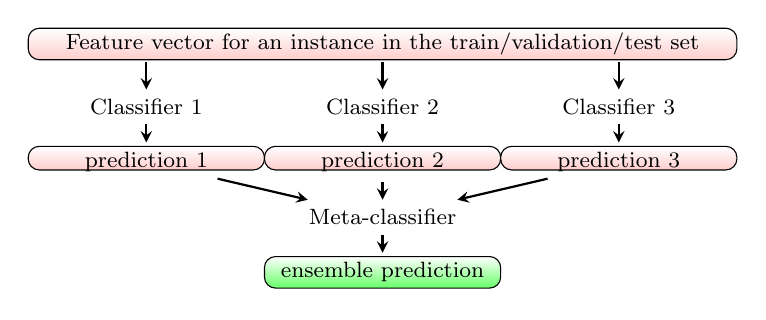
\begin{tikzpicture}
[split/.style={rectangle,rounded corners,draw=black, top color=white, bottom color=red!20, thin, inner sep=0.25em, minimum size=0.1em, text centered},
classical/.style={thick,->,shorten >=0pt,shorten <=0pt,>=stealth},
flow/.style={thick, gray, decoration={markings,mark=at position
   1 with {\arrow[thick,gray]{ triangle 60}}},
   double distance=6.5pt, shorten >= 6.5pt,
   preaction = {decorate, gray},
   postaction = {draw,line width=7pt, gray,shorten >= 6.3pt}},]
\draw[split] (0,1.6) rectangle (9,2.0); 
\node[draw=none] (1s) at (1.5,1.7){};
\node[draw=none] (2s) at (4.5,1.7){};
\node[draw=none] (3s) at (7.5,1.7){};

\node[draw=none,inner sep=1pt]  at (4.5,1.8) {\footnotesize Feature vector for an instance in the train/validation/test set};  

% third row
%\draw[split,bottom color=yellow!50] (9.2,1.1) rectangle (11.2,1.6); 
%\node[draw=none,inner sep=1pt]  (tv) at (10.2,1.3) {\footnotesize Test/Validation};

\node[draw=none] (1) at (1.5,1){\footnotesize Classifier 1};
\node[draw=none] (2) at (4.5,1){\footnotesize Classifier 2};
\node[draw=none] (3) at (7.5,1){\footnotesize Classifier 3};

\draw[classical] (1s) to (1);
\draw[classical] (2s) to (2);
\draw[classical] (3s) to (3);

%\draw[classical] (tv) to (3c);
%\draw[classical] (tv) to (2c);
%\draw[classical] (tv) to (1c);

\draw[split] (0,0.2) rectangle (3,0.5); 
\draw[split] (3,0.2) rectangle (6,0.5); 
\draw[split] (6,0.2) rectangle (9,0.5); 

\node[draw=none] (1p) at (1.5,0.3) {\footnotesize prediction 1};
\node[draw=none] (2p) at (4.5,0.3) {\footnotesize prediction 2};
\node[draw=none] (3p) at (7.5,0.3) {\footnotesize prediction 3};


% fifth row
\node[draw=none] (a) at (4.5,-0.4) {\footnotesize Meta-classifier};
\draw[split, bottom color=green!60] (3,-1.3) rectangle (6,-0.9); 
\node[draw=none] (ap) at (4.5,-1.1) {\footnotesize ensemble prediction};


\draw[classical] (1) to (1p);
\draw[classical] (2) to (2p);
\draw[classical] (3) to (3p);
\draw[classical] (1p) to (a);
\draw[classical] (2p) to (a);
\draw[classical] (3p) to (a);
\draw[classical] (a) to (ap);

%\draw[split] (2,0.1) rectangle (8,0.6); 
%\draw[split,bottom color=red!50] (0,0.1) rectangle (2,0.6); 
%\draw[split,bottom color=yellow!50] (8.2,0.1) rectangle (10,0.6); 
%
%\node[draw=none,inner sep=1pt]  at (4,0.3) {\footnotesize Train};  
%\node[draw=none,inner sep=1pt,text width=1cm]  at (0.7,0.3) {\footnotesize Validation}; 
%\node[draw=none,inner sep=1pt]  at (9,0.3) {\footnotesize Test};

\end{tikzpicture}}

\end{frame}


\begin{frame}[fragile]
\frametitle{Agenda}   % expectation: 33 slides + title and agenda, 11 slides per chunk
\begin{itemize}
\item \textcolor{gray}{Model Selection
\item Model Averaging
\item Ensembles: Bagging
\item Ensembles: Boosting and Stacking}
\item Tree-based Models  % decision trees effectively make the selection decisions on the fly; random forests then are ensembles. Maybe trees should be discussed before committees?
\item \textcolor{gray}{Conditional Mixture Models  % this may be in the next "lecture"?
\item Ensembles of Humans}  
\end{itemize}
\end{frame}



\begin{frame}
\frametitle{Decision Trees}

\begin{tikzpicture}
\node[draw] at (8,1.3) {Weight $>$ 5kg};
\draw(8,1) -- (6,0);
\node[draw=none] at (6.4,0.5) {true};
\draw(8,1) -- (10,0);
\node[draw=none] at (9.6,0.5) {false};

\node[draw] at (6,-0.3) {A: Dog};

\node[draw] at (10,-0.3) {Height $<$15cm};
\draw(10, -0.6) -- (8,-1.6);
\draw(10, -0.6) -- (12,-1.6);
\node[draw=none] at (8.3,-1.1){false};
\node[draw=none] at (11.6,-1.1){true};
\node[draw] at (8,-1.9){B: Dog};
\node[draw] at (12,-1.9){C: Cat};

\draw[style={very thick, ->, >=stealth'}](13,-2) -- (13,1.5);
\draw[style={very thick, ->, >=stealth'}](13,-2) -- (17,-2);
\draw(15,-2) -- (15,1.5);
\draw(13,0) -- (15,0);
\node[draw=none] at (15,-2.4){weight};
\node[draw=none] at (12.4,1.2){height};

\node[draw=none] at (16,0){A: Dog};
\node[draw=none] at (14,1){B: Dog};
\node[draw=none] at (14,-1){C: Cat};

\end{tikzpicture}

\end{frame}


\begin{frame}
\frametitle{Random Forest -- Adapting Bagging to Trees}
\begin{itemize}
%\item Applies a modified form of bagging to decision trees
\uncover<2->{\item With bagging, base models make similar splits on the same features -- the strongest predictors -- meaning their errors become correlated %recall that combination methods work well if the errors are uncorrelated
}
\uncover<3->{\item Random forest modifies the training procedure for each tree, $m$:
\begin{enumerate}
\item Randomly sample $N$ data points with replacement from a training set with $N$ data points.
\item Learn the tree using the greedy CART algorithm but when determining each split, consider only $d \ll D$ randomly-chosen features. % d is much less than D
\end{enumerate}}
\uncover<4->{\item As with bagging, combine predictions by taking mean/majority vote.}
\uncover<5->{\item Extremely effective in many applications (see Murphy (2012), Machine Learning: A Probabilistic Perspective, Section 16.2.5)}
\end{itemize}
\end{frame}

\begin{frame}[fragile]
\frametitle{Agenda}   % expectation: 33 slides + title and agenda, 11 slides per chunk
\begin{itemize}
\item \textcolor{gray}{Model Selection
\item Model Averaging
\item Ensembles: Bagging
\item Ensembles: Boosting and Stacking
\item Tree-based Models}  % decision trees effectively make the selection decisions on the fly; random forests then are ensembles. Maybe trees should be discussed before committees?
\item Conditional Mixture Models  % this may be in the next "lecture"?
\item \textcolor{gray}{Ensembles of Humans}  
\end{itemize}
\end{frame}


\begin{frame}
\frametitle{Recap}
\begin{itemize}
\item Model selection: choose the right model for the whole dataset $\rightarrow$ \emph{hard selection}
\item Bayesian model averaging (BMA): probabilistically select the right model for the whole dataset $\rightarrow$ \emph{soft selection}
\item Decision trees: split the feature space and model each region by one leaf node $\rightarrow$ \emph{hard selection depending on features}
\uncover<2->{\item Conditional mixture models: perform a soft, probabilistic split of the feature space $\rightarrow$ \emph{soft selection depending on features}}
%\emph{combine} models 
%\item Mixture of experts: probabilistically weight the models depending on inputs --> \emph{combine depending on features}
\end{itemize}
\end{frame}

%\begin{frame}
%\frametitle{Conditional Mixture Models}
%\begin{itemize}
%\item Similar to the mixture models we saw in earlier lectures
%\item For regression or classification, rather than clustering
%\begin{itemize}
%\item Target variable $t$
%\item Feature vector $\bs x$
%\item Component density $\bs\pi$
%\item Parameters of observation distribution $\bs\phi$
%\item Goal: estimate $p(t | \bs x, \bs\phi, \bs\pi)$
%\item Learn parameters using EM
%\end{itemize}
%\item Each data point is generated from one mixture component as in the Gaussian mixture model (GMM).
%\end{itemize}
%\end{frame}
%
%
%\begin{frame}
%\frametitle{Conditional Mixture Models}
%\begin{itemize}
%\item Predictive posterior: $p(t_n |x_n,\bs\phi,\bs\pi) = \sum_{k=1}^K \pi_k p(t_n | \bs x_n, \bs \phi_k)$
%\item Type of distribution for $p(t_n | \bs x_n, \bs \phi_k)$ 
%depends on the data types of $t_n$ and $\bs x_n$
%\item e.g., Gaussians for regression
%\item e.g., logistic model for classification.
%\item Allows us to model multimodal data:
%\end{itemize}
%\centering
%\includegraphics[width=0.7\textwidth]{conditional_density_plot}
%
%\footnotesize See Bishop (2006), 14.5.1 and 14.5.2.
%\end{frame}


\begin{frame}
\frametitle{Mixture of Experts}
\begin{itemize}
\item Each data point is processed by a weighted combination of specialised 'expert' models
\item Weights: probabilities that depend on the features $\bs x_n$ of the data point 
 %possibly a combination of models as in conditional mixture model.
\uncover<2->{\item Think of medical diagnosis: based on the patient's symptoms, a GP refers the patient to a specialist}
\uncover<3->{\item If they are unsure what is causing the symptoms, they may send the 
patient to multiple specialists for examination. }
\uncover<4->{\item Similarly, some inputs $\bs x_n$ may require a combination of expert models}
\uncover<5->{\item Contrast with decision trees,  which assign each data point to a single leaf node}
\end{itemize}
\end{frame}


\begin{frame}
\frametitle{Mixture of Experts}
\centering
Imagine we would like to learn a model of this function:
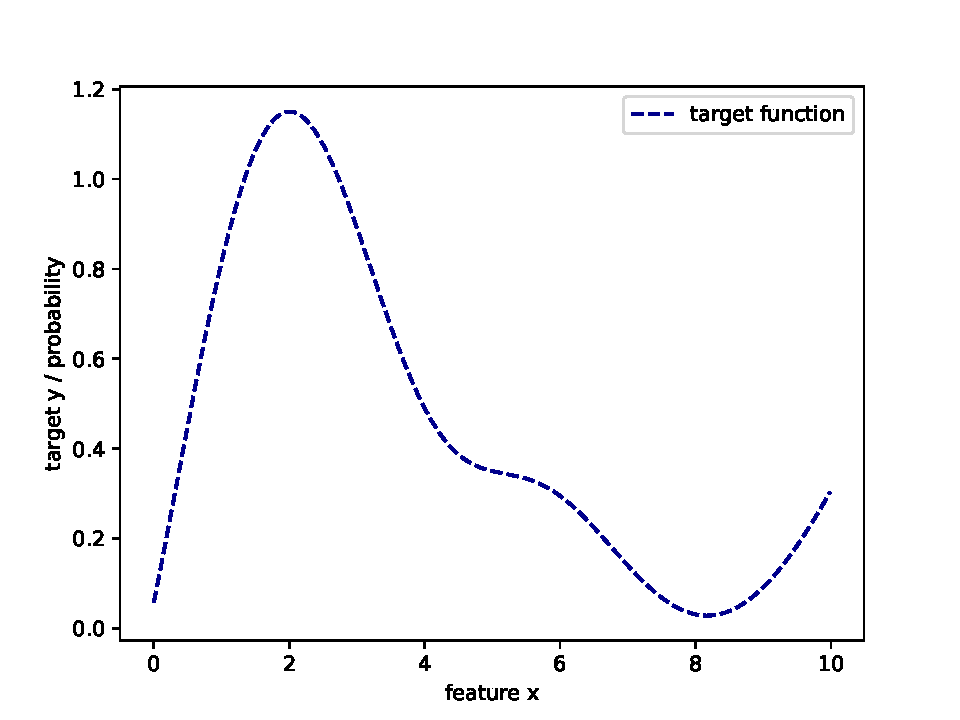
\includegraphics[width=0.8\textwidth]{../figures/MoE_sketch1}
% regression problem, x_n along the x axis, t along the y-axis.
% in this case, only a single expert is required to deal with each part of the input space. 
\end{frame}

\begin{frame}
\frametitle{Mixture of Experts}
\centering
We have two expert models: model 1 is close to our target on the left, model 2 is close to our target on the right. 
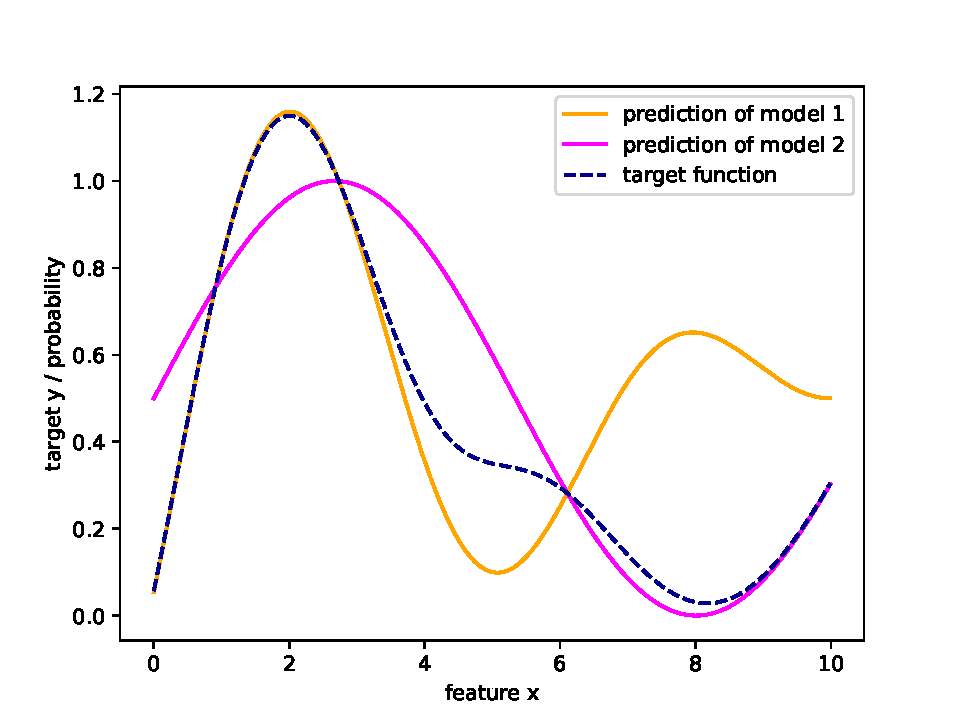
\includegraphics[width=0.8\textwidth]{../figures/MoE_sketch2}
% regression problem, x_n along the x axis, t along the y-axis.
% in this case, only a single expert is required to deal with each part of the input space. 
\end{frame}


\begin{frame}
\frametitle{Mixture of Experts (MoE)}
\centering
MoE reproduces the target function by learning weights for each model and taking a weighted sum of their predictions.
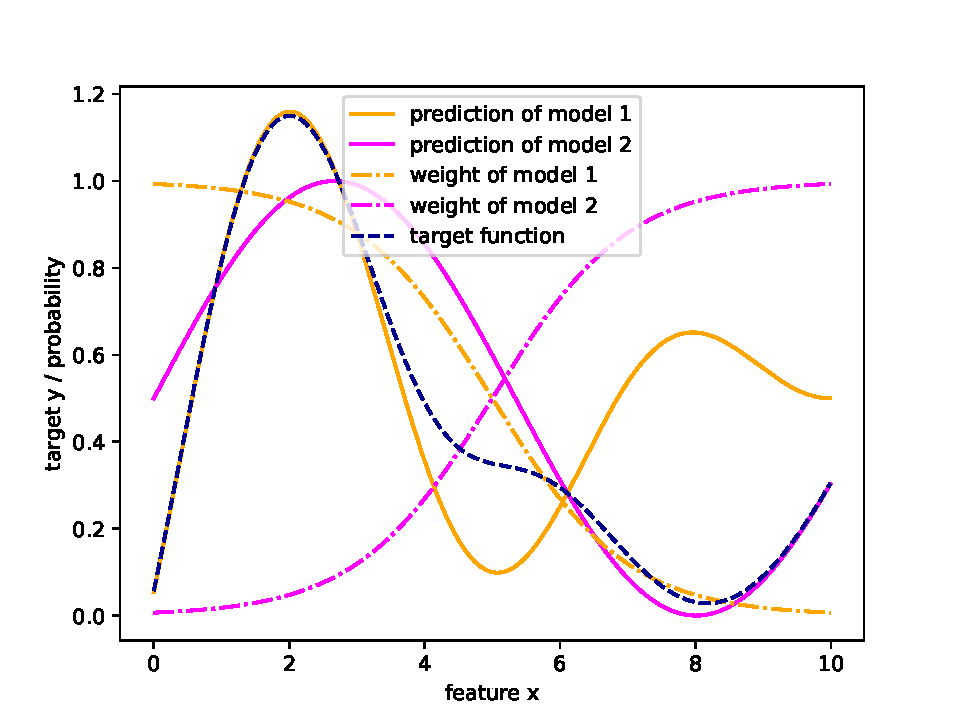
\includegraphics[width=0.8\textwidth]{../figures/MoE_sketch3}
% regression problem, x_n along the x axis, t along the y-axis.
% in this case, only a single expert is required to deal with each part of the input space. 
\end{frame}


\begin{frame}
\frametitle{Mixture of Experts}
\begin{itemize}
\item Goal: predict target variable $t_n$ given features $\bs x_n$
\item Component distribution 
 depends on input feature vector $\bs x_n$.
\begin{equation}
p(t_n | \bs x_n, \bs \phi, \bs\pi) = \sum_{k=1}^K \pi_k(\bs x_n) p(t_n | \bs x_n, \bs\phi_k)
\end{equation}
\item $\pi_k(\bs x_n)$ is the weight for model $k$ in a combination of models.
\item The weights can be learned as part of EM (see Bishop 14.5.3 for more)
\end{itemize}
\end{frame}


%%%%%%%%%%%%%%%%%%%%%%%%%%%%%%%%%%%%%%%%%%%%%%%%%%%%%%%%%%%%%%%%%%%%%% 
\begin{titledslide}{Reading}

  \begin{itemize}
  \item Bishop Chapter 14
  \item Murphy \S18.2--\S18.5.3
  \end{itemize}
  
  
\end{titledslide}
%%%%%%%%%%%%%%%%%%%%%%%%%%%%%%%%%%%%%%%%%%%%%%%%%%%%%%%%%%%%%%%%%%%%%%
\begin{titledslide}{Problems and quizzes}

  \begin{itemize}
  \item Problems:
    \begin{itemize}
    \item Bishop 14.2
    \item Bishop 14.3
    \end{itemize}
  \item Quizzes:
    \begin{itemize}
    \item Week~8: Model Selection and Averaging
    \item Week~8: Ensembles
    \item Week~8: Conditional Mixture Models
    \end{itemize}
  \end{itemize}
  
\end{titledslide}
%%%%%%%%%%%%%%%%%%%%%%%%%%%%%%%%%%%%%%%%%%%%%%%%%%%%%%%%%%%%%%%%%%%%%%
\bibliographystyle{alpha}
\bibliography{../ml}

\end{document}
